%%
%% 2020 - 08 -03 φ
%%

\section{Kombinatorik}
Die Kombinatorik befasst sich damit, wie viele Möglichkeiten für
verschiedene Konstellationen zur Wahl stehen.

Als Einstiegsbeispiel dient die folgende Wanderung:

\vspace{5mm}

\bbwGraphic{12cm}{geso/stoch/img/wanderung.png}

Auf wie viele Arten kann der Wanderer von Wesen (im Westen) nach Obertal (im Osten) gelangen, wenn er ausschließlich von West nach Ost wandern will?

Die Antwort kann durch Abzählen (oder eine Kombination von Abzählen und Multiplizieren) gefunden werden:

\TNT{2.4}{$3\cdot{}(1+(2\cdot3)) + 3 = 24$ Möglichkeiten. Mögliche
  Erklärung: Bis «L» sind 3 Wege offen. Bis «R» sind total 3*2 + 1,
  also sieben Wege möglich. Um nach «O» zu gelangen sind nun 7*3 + die
  drei Wege ab Lisibach und dann direkt, also total 24 Wege möglich. Parallele Wege werden addiert;
  serielle Wegmöglichkeiten multiplizieren sich.}

\newpage
\subsection{Variation mit Wiederholung (Produktregel)}
Ein Zahlenschloss hat vier Ringe und auf jedem Ring sind die Zahlen
von 0 - 5 einstellbar. Also pro Ring sechs Möglichkeiten.
Wie viele Variationen gibt es im ganzen für dieses Zahlenschloss?

\bbwCenterGraphic{5cm}{geso/stoch/img/zahlenschloss.jpg}

\TNT{7.2}{
Jeder Ring hat 6 Möglichkeiten. Somit habe ich am 1. Ring sechs
Varianten. Für jede dieser Varianten habe ich für den 2. Ring auch
sechs Varianten. Insgesamt also

$n$ = Anzahl Objekte zur Auswahl; diese müssen nicht unbedingt gewählt werden (hier 6 Ziffern)

$k$ = Vorgegebene Anzahl geordnete auszuwählende Objekte (hier 4, weil es 4 Ringe hat)

$N$ = Anzahl Variationen

$$N = n^k = 6^4$$
}

Dieses Experiment entspricht im Urnenmodell dem...
\begin{gesetz}{...Ziehen \textbf{mit} Zurücklegen.}{}
Bei diesem Urnenmodell kann jeder Zug unabhängig vom
vorangehenden wieder alle Werte annehmen. Die \textbf{Reihenfolge} der gewählten Kugeln ist hier \textbf{wesentlich}. Für $k$ Züge aus genau $n$
Kugeln, die alle verschieden sind, gibt es $N$ Möglichkeiten:
$$N = n^k$$
\end{gesetz}

\begin{definition}{Variation}{}\index{Variation}
Eine \textbf{Variation} ist eine \textbf{geordnete} Stichprobe.
\end{definition}
\newpage

\subsection*{Referenzaufgabe Zahlenschloss}
Ein Zahlenschloss wie eben soll gebaut werden. Dabei hat jeder Ring
die Ziffern von 0 bis 6 (also insgesamt 7 Ziffern).
Das Schloss soll mindestens 20\,000 Variationen anbieten. Wie viele
Ringe muss ich nehmen?

\TNT{9.6}{
Hier ist die Anzahl Ringe (also das $k$) unbekannt. Gegeben sind

$$n=7$$
$$N\ge{}20\,000$$
Die Formel lautet
$$N\ge{}n^k$$
$$20\,000\ge{}7^k$$
Wo wären die beiden Terme gleich?
$$20\,000 = 7^k$$
Durch Logarithmieren erhalten wir:
$$k = \log_7(20\,000)\approx 5.089$$
Damit müssen wir mind. \textbf{6 Ringe} einsetzen, denn bei 5 Ringen erhalten
wir erst 16\,807 Variationen.
}%% END TNT


\subsection*{Aufgaben}
\aufgabenfarbe{Kompendium S. 46 Kap. 5.5.1 Aufg. 16. a)}
\newpage


\subsection{Permutationen (Fakultät)}\index{Permutation}\index{Fakultäten}
Lateinisch «permutare» = vertauschen

Hanna und Igor fahren Bus. Die beiden für sie reservierten Plätze sind
nebeneinander, doch nur einer davon ist ein Fensterplatz. Auf wie
viele Arten können sich die beiden Personen auf die beiden Plätze
verteilen?

\TNT{2.4}{Genau auf zwei Arten: Entweder ist
Hanna am Fenster, oder Igor.\vspace{12mm}}

Das Problem ist etwas komplizierter, wenn nun Hanna, Igor mit Jana
eine Flugreise machen. Die drei reservierten Plätze sind wieder
nebeneinander. Ein Platz ist am Fenster, einer zum Gang und der dritte
Platz ist zwischen den beiden anderen. Auf wie viele Arten können nun
Hanna, Igor und Jana ihre Plätze wählen?

\TNT{3.6}{6 Varianten. Jede der drei Personen
am Fenster ergibt drei Hauptvarianten, dann jede der verbleibenden
beiden zum Gang hin; Ergo: $3\cdot{}2$}

Machen Sie die selbe Überlegung noch mit vier Personen\footnote{Ach ja: Die vierte Person ist Karl.} und vier
Plätzen...

\TNT{2.8}{24 = 4!\vspace{28mm}}

... und mit fünf Plätzen und fünf Personen\footnote{Die fünfte Person heißt übrigens Lena, auch wenn es für die Berechnung keine Rolle spielt.}.

\TNT{3.2}{120 = 5!\vspace{30mm}}
\newpage


\subsubsection{Fakultät als Operation}\index{Fakultät}
\TRAINER{Youtube Video als Vorbereitung MatheMai (S. Wiki):\\\texttt{https://www.youtube.com/watch?v=cVCBNVDav3U}}

Ganz allgemein gilt: Bei $n$ Personen auf $n$ Plätzen gibt es

$$n\cdot{} (n-1) \cdot{} (n-2) \cdot{} (n-3) \cdot{} (n-4) \cdot{}
... \cdot{} 2 \cdot{} 1$$

Möglichkeiten.

Diese Rechnung ist im Taschenrechner unter der Operation ``Fakultät''
bekannt und wird üblicherweise mit der Taste \fbox{n!} bezeichnet. Auf
Ihrem Rechner ist es die Taste \tiprobutton{ncrnpr}.

Berechnen Sie die Fakultät von 3, 4, 5 und 20 mit dem Taschenrechner.

\TNT{3.2}{\vspace{32mm}}

Auf wie viele Arten können Sie sich als Klasse in Ihre Bänke
verteilen? Machen Sie die Überlegung so, wie es aussehen würde, wenn es keine leeren Plätze gäbe.

\TNT{5.2}{Wenn es keine leeren Plätze hat, entspricht die Anzahl der
Möglichkeiten der Fakultät. $n$ = Anzahl Schüler = Anzahl Plätze, dann
gilt $n!$ = Anzahl mögliche Sitzordnungen.
\vspace{32mm}
}

Dies entspricht im Urnenmodell dem ...
\begin{gesetz}{...Ziehen \textbf{ohne} Zurücklegen.}{}
In diesem Urnenmodell entspricht die Fakultät einer Urne mit $n$ Kugeln, die
alle verschieden sind. Alle $n$ Kugeln werden gezogen. Wie viele
Reihenfolgen sind möglich?
$$N = n\cdot{} (n-1) \cdot{} (n-2) \cdot{} (n-3) \cdot{}
(n-4) \cdot{} ... \cdot{} 3\cdot{} 2 \cdot{} 1 = n!$$
\end{gesetz}
\newpage


Ein alter Bekannter (optional):

\vspace{3mm}

\begin{bemerkung}{Summenzeichen}{}
Erinnern Sie sich an das Summenzeichen? Berechnen
Sie $$\sum_{n=0}^{15}\frac{1}{n!} = \frac{1}{0!} + \frac{1}{1!}
+ \frac1{2!} + \frac1{3!} + \frac1{4!} + ... + \frac1{15!}$$ Das Summenzeichen finden Sie unter
der Taste \tiprobutton{math}\tiprobutton{5}.\footnote{Gönnen Sie sich
ein Glas süßen Sirup, während Ihr Taschenrechner diese Summe für Sie berechnet.}
\end{bemerkung}

Erinnern Sie sich auch an dieses Resultat? \TRAINER{$= e \approx 2.718281828459045$}



\subsection*{Aufgaben}
\aufgabenfarbe{Kompendium Kap. 5.5.1 Aufg. 15}
\newpage


\subsection{Variation ohne Zurücklegen}\index{Variation!ohne Zurücklegen}
Stellen wir uns vor, wir könnten sechs Kunstbände (Bücher) in ein schmales
Regal stellen. Mehr geht nicht, weniger wollen wir nicht.
Nun haben wir zehn solcher Bücher zur Auswahl. Auf wie viele Arten können wir nun sechs Bücher in unser Regal einordnen?

\TNT{6}{
Für das erste Buch haben wir zehn Möglichkeiten. Wenn das Buch da mal steht, haben wir für das zweite Buch nur noch neun Möglichkeiten.
Schlussendlich bleiben $N$-Möglichkeiten:
$$N=10\cdot{}9\cdot 8\cdot 7\cdot 6\cdot 5 = \frac{10\cdot 9\cdot 8\cdot 7\cdot 6\cdot 5\cdot 4\cdot 3\cdot 2\cdot 1}{4\cdot 3\cdot 2\cdot 1} = \frac{10!}{4!}$$
\vspace{20mm}
}%% END TNT

Oder als Formel:
\begin{gesetz}{Ohne Zurücklegen / Reihenfolge wesentlich}{}
Es seien
$n = $ Anzahl Objekte der Auswahl (oben die Anzahl der Bücher), ev. nicht jedes wird gewählt\\
$k = $ Anzahl auszuwählende geordnete Objekte (die Anzahl Plätze im Regal, jeder Regalplatz wird besetzt)\\
$N = $ Anzahl der Möglichkeiten\\

$$N =\frac{n!}{(n-k)!}$$
\end{gesetz}

Veranschaulichung (2 aus 5):

\begin{tabular}{c|c|c|c|c}
12 & 21 & 31 & 41 & 51\\
13 & 23 & 32 & 42 & 52\\
14 & 24 & 34 & 43 & 53\\
15 & 25 & 35 & 45 & 54\\
\end{tabular}

Das sind fünf Blöcke mit je vier Objekten = $5\cdot{}4 = \frac{5!}{(5-2)!}$.
\newpage

\begin{bemerkung}{}{}
Wenn wir alle $n$ Objekte geordnet auswählen, so erhalten wir
$\frac{n!}{(n-n)!} = n!$, was dem bereits bekannten Spezialfall der \textbf{Permutation}
entspricht.
\end{bemerkung}


\GESO{%%
\begin{bemerkung}{}{}
Die Variation ohne Zurücklegen kann mit dem Taschenrechner mit «nPr» erreicht werden.
Eine \textbf{Rangliste}\index{Rangliste} von 3 Skifahrern (1., 2. und 3. Platz) aus 20
Mitfahrenden ist also $$\frac{20!}{(20-3)!}\TRAINER{=6840}$$ und kann auf dem
Taschenrechner mit der Taste «nPr» \tiprobutton{ncrnpr} erreicht
werden\footnote{Die Taste muss dabei drei Mal gedrückt werden!}.
\end{bemerkung}
}%%% end GESO

\begin{gesetz}{Variation ohne Wiederholung}{}
Bei $n$ Objekten zur Auswahl und $k$ geordnet ausgewählten Objekten davon, ist immer
$$n \ge{} k.$$
\end{gesetz}
\newpage

\subsubsection{Freie Plätze?}

Wie viele Möglichkeiten hat eine Klasse mit $n$ Lernenden, sich auf
$n+1$ Plätze zu verteilen?

\TNT{2.4}{Hier stellt man sich einfach einen ``Phantom-Schüler'' vor,
der unsichtbar auf der leeren Bank sitzt. Somit gilt auch hier: Die
Anzahl der Möglichen Sitzordnungen = Fakultät der leeren Plätze = $(n+1)!$.}

Wie viele Sitzordnungen sind möglich, wenn es zwei oder mehr freie Plätze gibt?

\TNT{8}{Hier gibt es grundsätzlich zwei Betrachtungsweisen.

a) Wir stellen uns vor, dass wir $n$ Plätze haben. Davon bleiben $f$
frei. Nun zählen wir alle Schüler und die ``Phantomschüler'' zusammen, das ergibt
gerade die $n$ Plätze. Hier gibt es also $n!$ Varianten. Die $f$
Phantomschüler setzen sich aber auch für alle Variationen mit realen
Schülern auf $f!$ verschiedene Varianten hin. Somit müssen wir diese
Varianten wieder wegdividieren. Es bleiben total $\frac{n!}{f!}$ Varianten.

Varianten = $\frac{n!}{(n-k)!} = \frac{n!}{f!}$ mit $f = n-k$ (= Anzahl der «Phantomschüler»).

b) Wir stellen uns die Sitzbänke nummeriert vor und legen für jeden der
$n$ Nummern eine Kugel in eine Urne. Die $k$ Schüler stellen wir der Reihe
nach hin, und jede/r darf der Reihe nach eine Kugel (somit seine
Platznummer) auswählen. Somit verbleiben $n-k$ Kugeln in der Urne und
hier gilt das \textbf{Ziehen ohne Zurücklegen mit wesentlicher
Reihenfolge}:


Varianten = $\frac{n!}{(n-k)!}$.

}%% END TNT
\newpage

\begin{bemerkung}{«Plätze» ist nicht gleich «Stühle»}{}
Nicht immer sind die zur Verfügung stehenden Objekte die Personen und nicht immer wird die Reihenfolge durch die Plätze (Stühle) festgesetzt:


\begin{tabular}{|p{62mm}|c|p{55mm}|}\hline
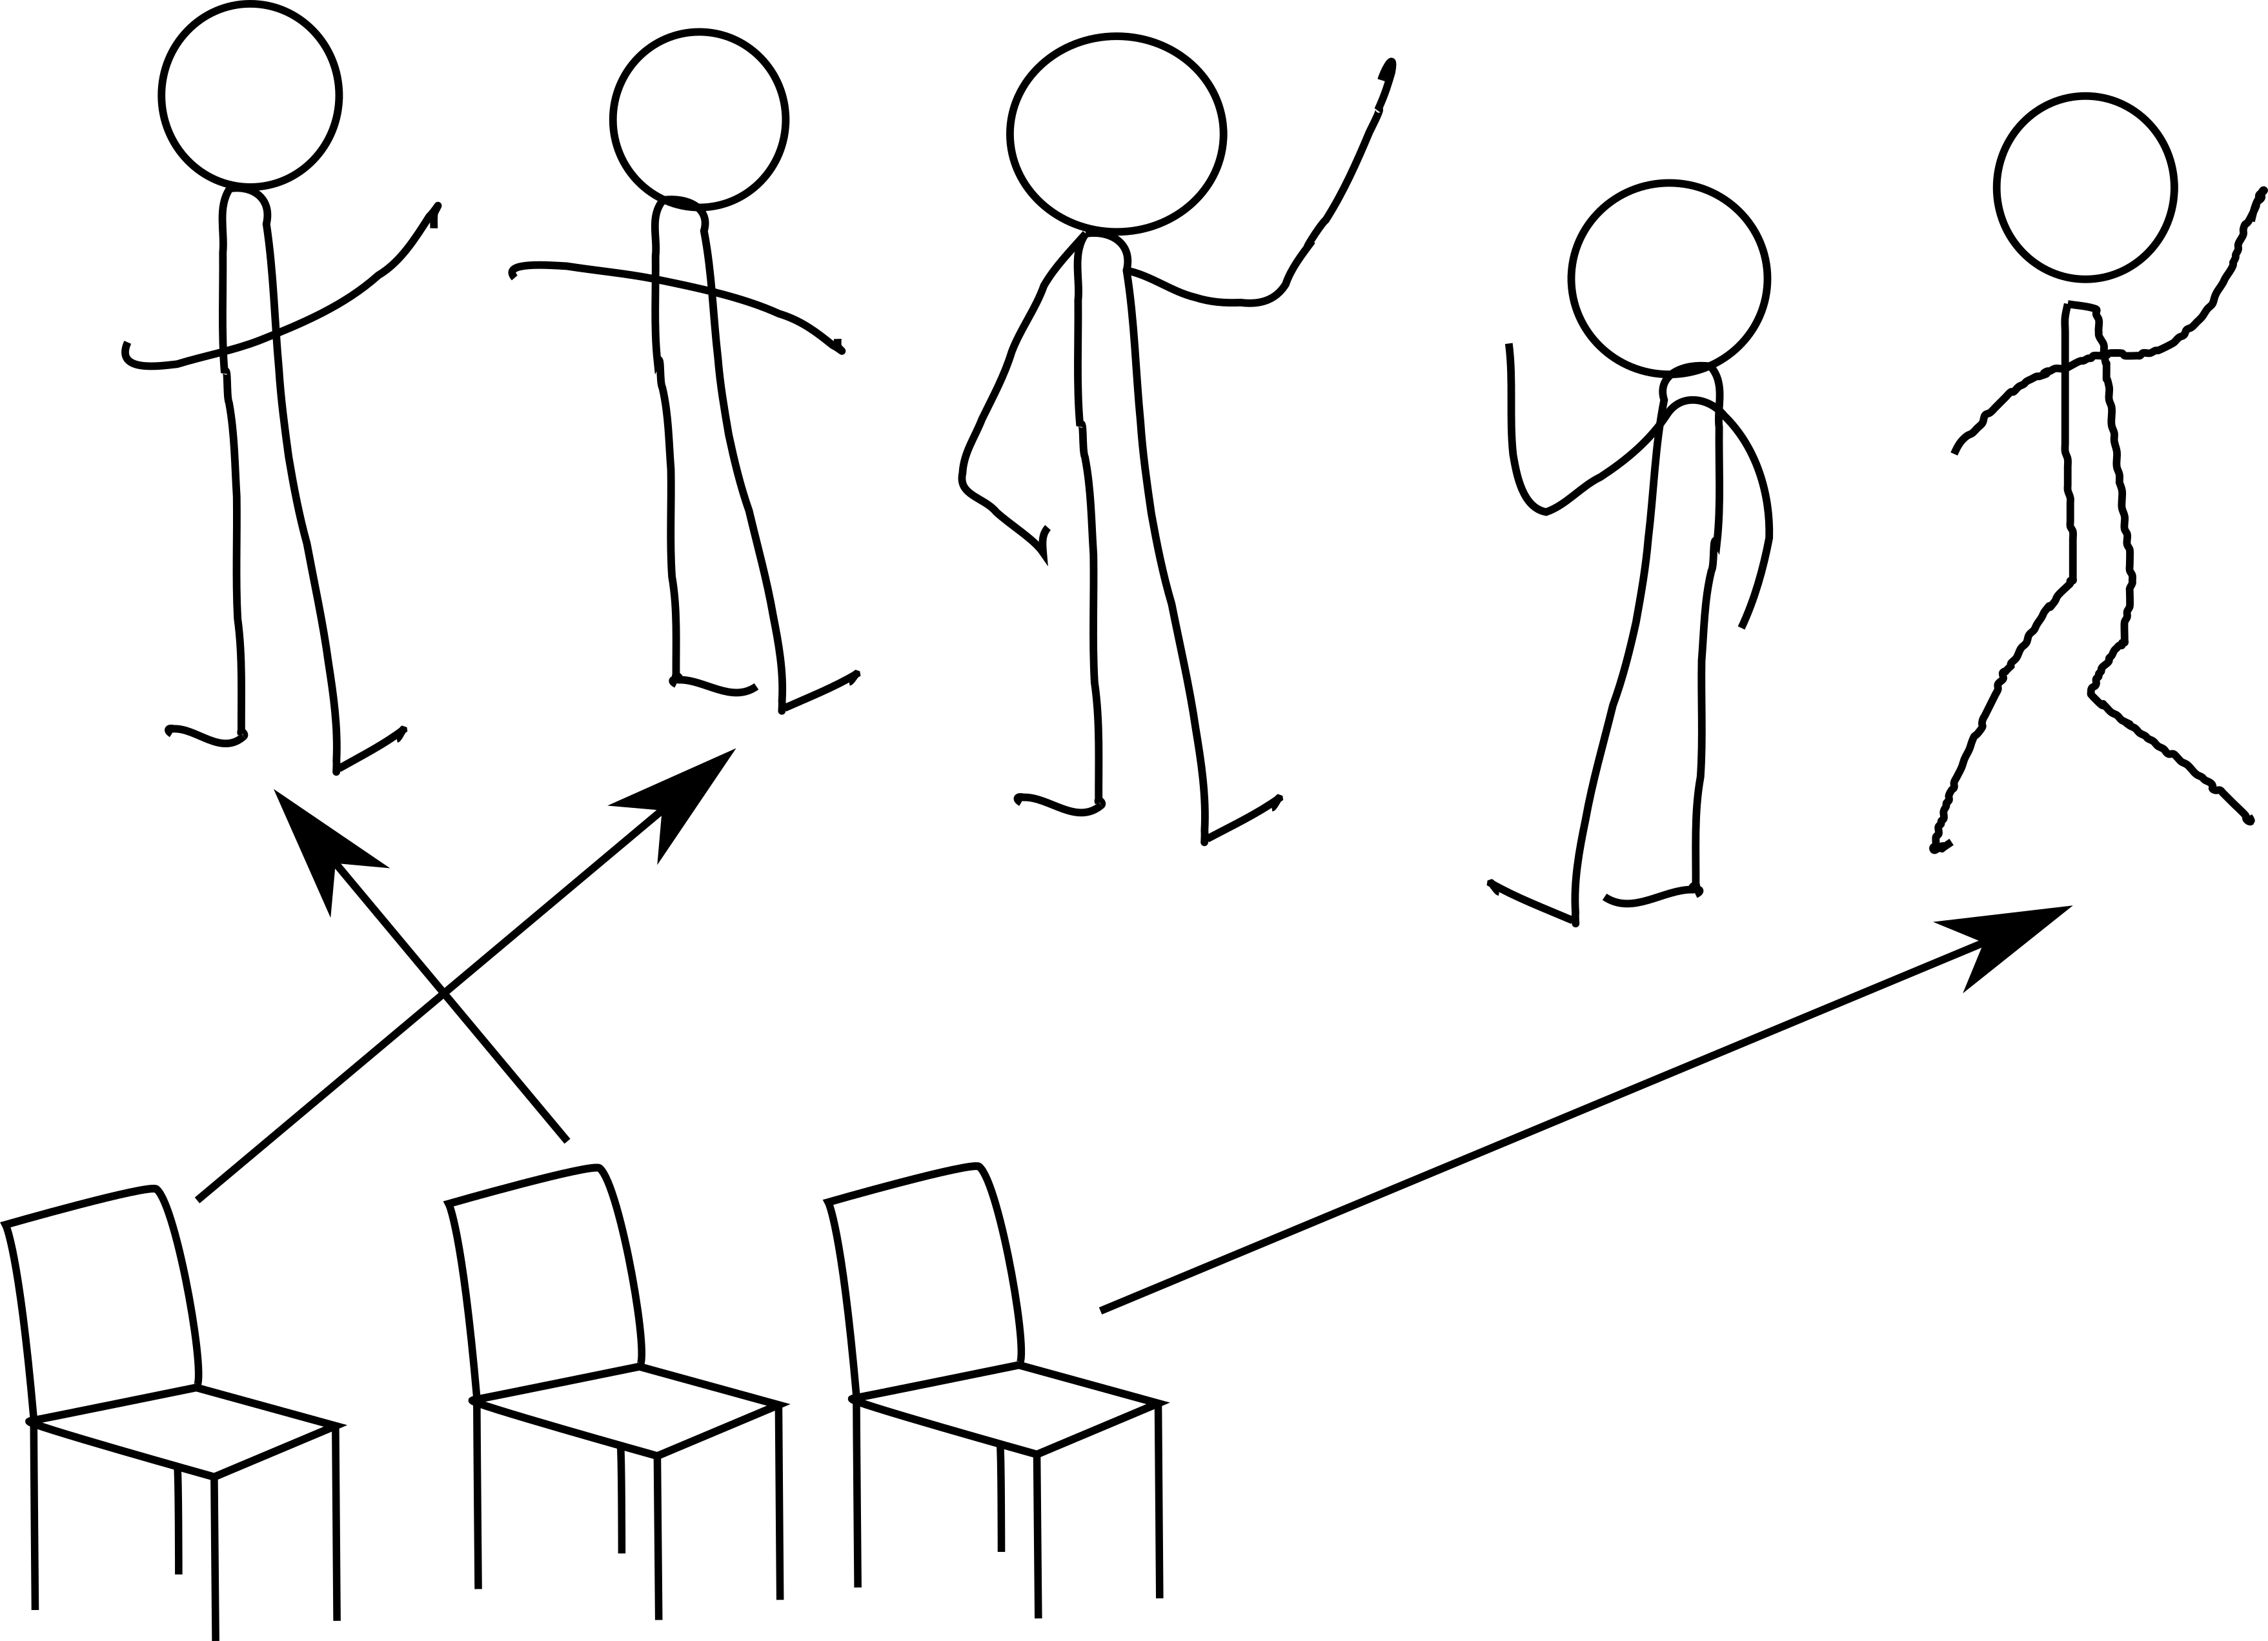
\includegraphics[width=5cm]{geso/stoch/img/fuenfPersonenAufDreiStuehle.png}
& \raisebox{20mm}{\parbox{40mm}{$$n=5$$ $$k=3$$}} & 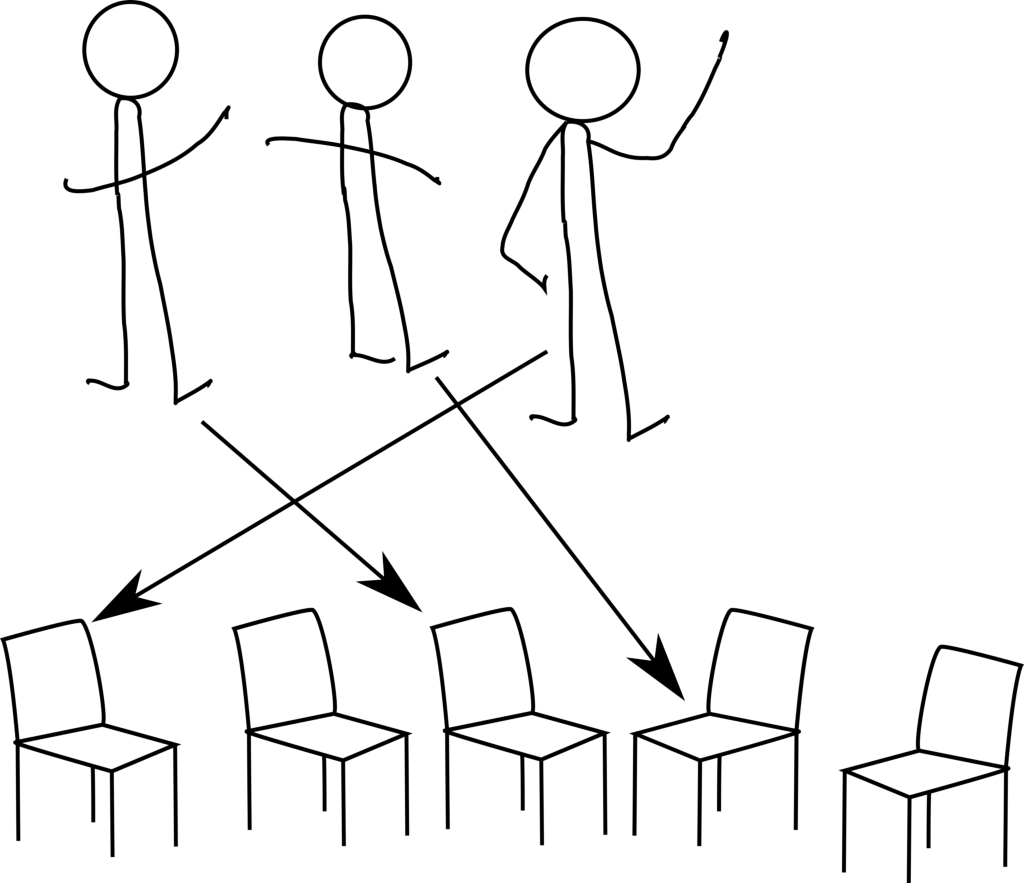
\includegraphics[width=5cm]{geso/stoch/img/dreiPersonenAufFuenfStuehle.png}\\\hline
Hier sind fünf Personen \textbf{zur Auswahl}, somit ist $n=5$. Die Ordnung wird als Reihenfolge der Stühle betrachtet $(k=3)$. &\raisebox{-10mm}{$N=\frac{5!}{(5-3)!}$}&
Hier sind fünf Stühle \textbf{zur Auswahl}, somit ist $n=5$. Die
Ordnung wird als Reihenfolge der Personen (\zB 1. Person auf Stuhl C)
betrachtet $(k=3)$.\\\hline
Im Urnenmodell bezeichnen fünf Kugeln die fünf Personen und ich ziehe \textbf{der Reihe nach} drei heraus, die ich in eben dieser Reihenfolge auf die Stühle setze. &
\raisebox{-35mm}{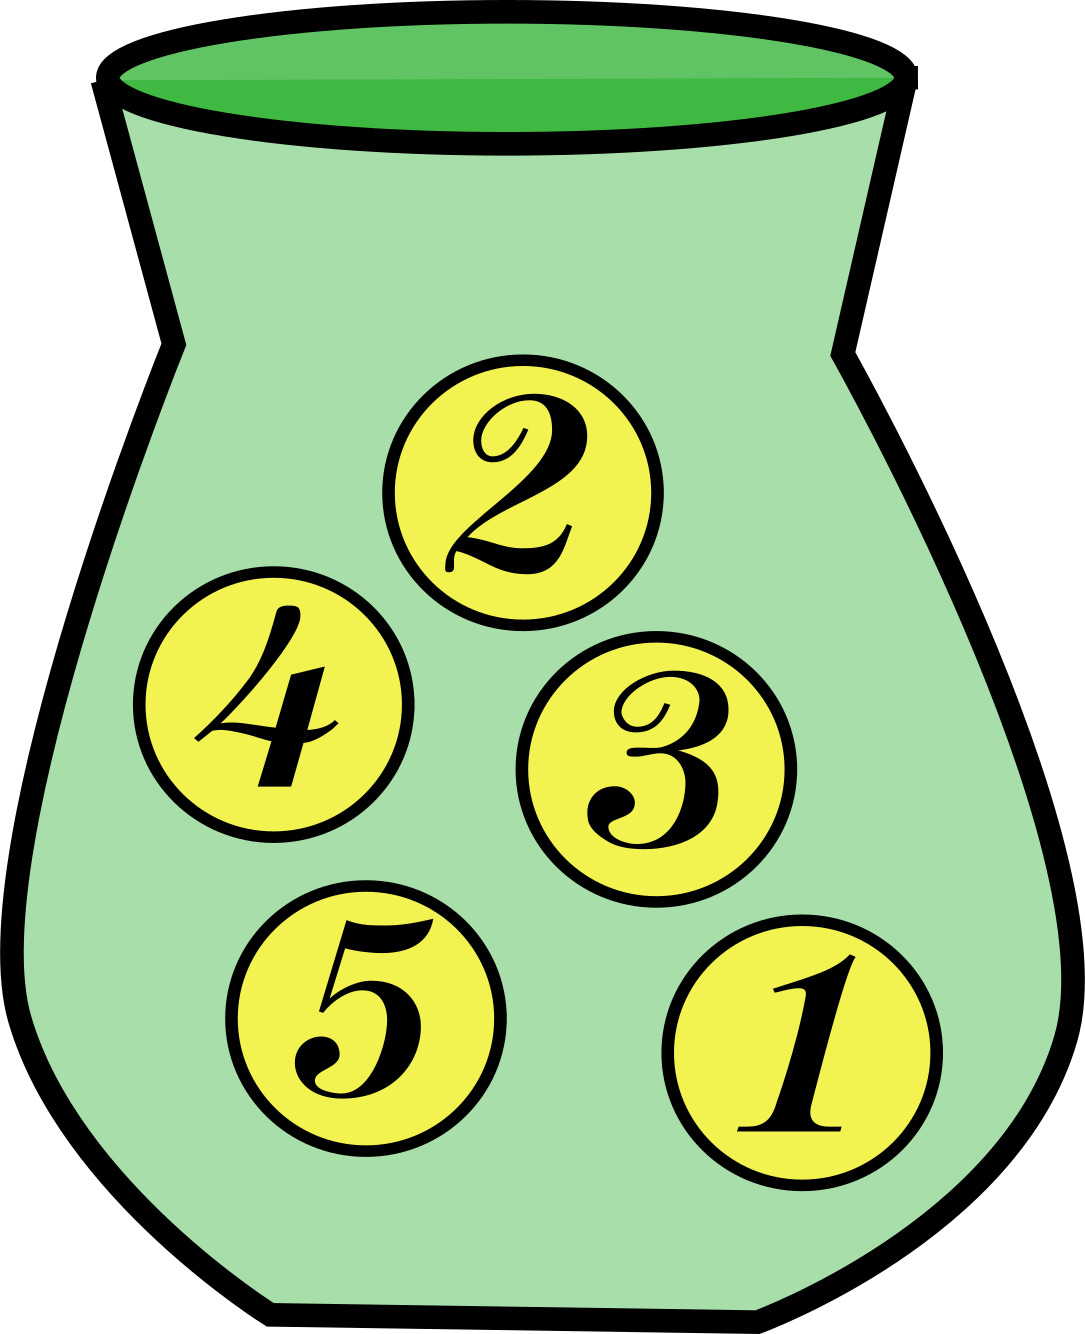
\includegraphics[width=3cm]{geso/stoch/img/urneFuenfKugeln.png}}&
Im Urnenmodell bezeichnen fünf Kugeln die fünf Stühle und ich ziehe \textbf{der Reihe nach} drei heraus, die ich in eben dieser Reihenfolge den Personen zuordne.\\\hline
Es wäre eine andere Problemstellung, für die 1. Person drei mögliche Stühle, für die 2. Person zwei Stühle und für die 3. Person den 3. verbleibenden Stuhl auszuwählen. Hier kämen die Personen 4 und 5 gar nie zum Sitzen und das Problem würde sich auf die Permutationen von 3 (also 3!) beschränken.&&\\\hline
\end{tabular}

\leserluft

Konvention: Das $n$ ist immer die größere der beiden Zahlen: $n > k$

\end{bemerkung}
\newpage

\subsection*{Aufgaben}

\aufgabenfarbe{Ein Zahlenschloss mit vier Ringen wird verdreht. Jeder
Ring hat alle Ziffern von 0..9 (also zehn Ziffern) als wählbare
Möglichkeiten. Auf wie viele Arten kann ich das Zahlenschloss
verdrehen, wenn jede Ziffer genau einmal vorkommen darf?}
\TNT{2.4}{1. Ring: 10 Möglichkeiten, 2. Ring 9, 3. Ring 8 und 4. Ring 7:
Also $10\cdot{}9\cdot{}8\cdot{}7 = \frac{10!}{(10-4)!} = 5040$}

\aufgabenfarbe{Das selbe Zahlenschloss wird so verdreht, dass eine
Ziffer dreimal und eine andere Ziffer einmal vorkommt. Wie viele Varianten
sind das?}
\TNT{2.4}{Es sind 360 Varianten. Nämlich 10 Varianten für die Ziffer,
die dreimal vorkommt, und noch 9 Varianten für die Ziffer, die genau
einmal vorkommt. Dies macht 90 Varianten zwei Ziffern so auszuwählen,
dass die erste Ziffer dreimal und die zweite Ziffer einmal
vorkommt. Nun haben wir für diese 90 Varianten aber immer vier
Möglichkeiten zu wählen, wo die einzelne Ziffer steht. Somit 10 mal 9
mal 4 = 360.}

\aufgabenfarbe{Das selbe Zahlenschloss wird so verdreht, dass eine
Ziffer maximal zweimal auftreten kann. Wie viele Varianten gibt es nun?}
\TNT{2.4}{Es sind 4670 Varianten. Dies geht am einfachsten mit
Abzählen. Von den Total 5040 Varianten fallen die zehn weg bei denen
alle Ziffern gleich sind und ebenso fallen die 360 weg, bei denen drei
gleiche Ziffern vorkommen (s. obige Aufgabe). Somit verbleiben $5040-10-360=4670$.
}


\aufgabenfarbe{Kompendium: S. 46 Aufg. 16. b)}

\newpage



%%%%%%%%%%%%%%%%%%%%%%%%%%%%%%%%%%%%%%%%%%%%%%%%%%%%%%%55

\subsection{Kombinationen}\index{Kombination}
Im Folgenden betrachten wir die Familie G. aus W.:
\begin{itemize}
\item Mutter, klein, dunkelhaarig
\item Vater, groß, blond
\item 1. Kind: Tochter, groß, blond, Teenager
\item 2. Kind: Sohn, klein, blond, Teenager
\item 3. Kind: Tochter, klein, dunkelhaarig (noch kein Teenager)
\end{itemize}

Die Familie hat gemerkt, dass es meist nicht nötig ist, alle Namen
aufzuzählen, wenn eine Teilmenge der Familie angesprochen werden soll:

\begin{itemize}
\item «Heute kochen die Blonden»
\item «Die Großen dürfen heute ausnahmsweise länger aufbleiben»
\item ...
\end{itemize}

\newpage
Beantworten Sie die folgenden Fragestellungen:
\begin{itemize}
\item Wie viele ``Teilmengen'', solcher \textbf{Kombinationen}, bestehend aus genau \textbf{drei} Familienmitgliedern sind möglich?

\TNT{1.6}{10\vspace{10mm}}

\item (optional) Suchen Sie zu zweit für jede «Dreiergruppe» der Familie G. eine
treffende Bezeichnung.

\TNT{4.4}{
  die drei Ältesten,
  Mutter und Männer (M\&Ms),
  keine Teenager,
  Mutter und Teenager,
  die «Damen»,
  die blonden,
  Vater und Töchter,
  Vater und beide Jüngsten,
  die Kinder,
  Vater und Teenager
  \vspace{30mm}
}% END TNT

\item (optional) Wie viele ``Teilmengen'', nicht nur mit drei Personen, gibt es in der
  fünfköpfigen Familie im Ganzen?
  \TNT{4}{$$N=2^5=32$$
    
    Entweder durchzählen: 0 oder alle gewählt: je eine Variante, 1 oder 4 gewählt: je 5 Varianten oder 3 oder 2 gewählt: je 10 Varianten

    Oder folgende Überlegung (Variation mit Wiederholung): Für jedes Familienmitglied hat es zwei Optionen a) ``dabei'', b) ``nicht dabei'' Somit haben wir $2^5$ Variationen ($k=5$ für jedes Familienmiglied muss ich die Entscheidung treffen. und $n=2$ die Entscheidungen ``dabei'', ``nicht dabei'' müssen aber nicht unbedingt beide vorkommen.
  }%% END TNT

\item (optional) Wie viele Teilmengen wären möglich in einer sechsköpfigen,
bzw. siebenköpfigen Familie? (6köpfig: \LoesungsRaum{$2^6=64$};
7köpfig: \LoesungsRaum{$2^7=128$})

\end{itemize}
\newpage


Die Anzahl der Möglichkeiten, drei Objekte aus einer Menge mit total
fünf Objekten auszuwählen, wird in der Mathematik mit dem
Binomialkoeffizienten angegeben:

\TNT{2}{$$N={5\choose 3} = 10$$} %% END TNT

Berechnet wird dies mit der Fakultät (Anzahl der Permutationen), indem
alle fünf Objekte permutiert werden. Wir erhalten so zu viele
Möglichkeiten. Wir dividieren die Zahl durch die Anzahl aller Permutationen der
gewählten Personen, aber auch durch die Anzahl aller Permutationen der
nicht gewählten Personen:

\TNT{2}{$$n={5\choose 3} = \frac{5!}{3!\cdot{} 2!}$$}%% END TNT
\newpage

\begin{definition}{Kombination}{}\index{Kombination!Definition}
Eine \textbf{Kombination} ist eine \textbf{un}geordnete Stichprobe.
\end{definition}

Wenn die Reihenfolge der Objekte keine Rolle spielt, gilt ganz
allgemein:

Die Anzahl der Möglichkeiten, $k$ Objekte aus einer Grundgesamtheit
von $n$ Objekten auszuwählen, ist gleich

\begin{definition}{Binomialkoeffizient}{}\index{Binomialkoeffizient!Definition}
$${n\choose k} = \frac{n!}{k!(n-k)!}$$
\end{definition}

Berechnen Sie gleich:
\begin{itemize}
\item $5\choose 3$\TRAINER{ = 10}
\item $5\choose 2$ (begründe) \TRAINER{  = 10, denn 3 Auswählen ist gleich
wie zwei nicht wählen!}
\item Swiss LOTTO (ohne den Stern) ${42\choose 6}$ \TRAINER{$ = 5\,245\,786$}
\end{itemize}


Diese Zahl wird Binomialkoeffizient genannt und kann mit dem
Taschenrechner einfach
mittels \tiprobutton{ncrnpr}\footnote{Zweimaliges Drücken der Taste:
Wählen Sie für den Binomialkoeffizienten ``nCr'', nicht ``nPr''.}
berechnet werden.


\begin{bemerkung}{}{}
Zur Begründung: Stellen Sie die $n$ Objekte in eine Reihe. Dazu gibt
es $n!$ Möglichkeiten. Nun dividieren wir die Vertauschungen der
gewählten Objekte ($k!$) und die Vertauschungen der nicht gewählten
Objekte $(n-k)!$ davon weg, es bleibt $\frac{n!}{k!(n-k)!}$.
\end{bemerkung}

\begin{gesetz}{}{}
Im Urnenmodell entspricht der Binomialkoeffizient dem Ziehen von $k$ Kugeln aus einer
Urne mit $n$ verschiedenen Kugeln. Die Reihenfolge der gewählten
Kugeln ist hier nicht relevant.
\end{gesetz}
\newpage

\subsubsection{Referenzaufgabe Euromillions}
Beim Glücksspiel «Euromillions» werden fünf aus 50 Zahlen und zwei aus zwölf Sternen angekreuzt. Auf wie viel Arten ist dies möglich?

\TNT{6}{${50 \choose 5} \cdot {12 \choose 2} = 139\,838\,160$\vspace{2cm}}
\newpage

\subsection{Zusammenfassung}
%%\bbwCenterGraphic{16cm}{geso/stoch/img/KombinatorikRLP.pdf}
$N = $
Anzahl Möglichkeiten, um $\color{red}k$ Elemente aus total $\color{blue}n$ Elementen auszuwählen.

\begin{tabular}{p{15mm}|p{80mm}|p{80mm}}
& $$\textrm{\textbf{mit} Wiederholung}$$ $$\textrm{(= mit
    Zurücklegen)}$$ & $$\textrm{\textbf{ohne}
    Wiederholung}$$ $$\textrm{(= ohne Zurücklegen)}$$\\\hline

%% Zeilentitel Variationen
\rotatebox[origin=rT]{90}{\makecell{\textbf{Variation}\\Reihenfolge wesentlich}}
&
%% Formeln
 \begin{center}{\fbox{$N={\color{blue}n}^{\color{red}k}$}}\end{center}
 Bsp.: Anzahl Wörter der Länge
 {\color{red}10}, die man aus {\color{blue}26} Buchstaben bilden kann: $${\color{blue}26}^{\color{red}10}
 \approx 1.41 \cdot{} 10^{14}$$
&
 \begin{center}{\fbox{$N = \frac{{\color{blue}n}!}{({\color{blue}n}-{\color{red}k})!}$}}\end{center}
 Bsp.: Anzahl Möglichkeiten, $\color{red}4$ Leute auf $\color{blue}
 10$ Sitzplätze zu verteilen.
 $$\frac{{\color{blue}10}!}{({\color{blue}10}-{\color{red}4})!} = 5040$$

 \\\hline

%% Zeilentitel Kombinationen
\rotatebox[origin=rT]{90}{\makecell{\textbf{Kombination}\\Reihenfolge irrelevant}}
&
%% Formeln
 \begin{center}$N = {{\color{blue}n}+{\color{red}k}-1 \choose {\color{red}k}}$\end{center}
 Bsp.: Anzahl Möglichkeiten, $\color{red}4$ Brote aus $\color{blue}10$ Sorten auszuwählen:
 $${{\color{blue}10}+{\color{red}4}-1 \choose {\color{red}4}} = 715$$
&
 \begin{center}{\fbox{$N={{\color{blue}n} \choose {\color{red}k}}$}}\end{center}
 Bsp.: Anzahl Möglichkeiten, $\color{red}4$ Karten aus {\color{blue}10} zu ziehen: $${{\color{blue}10} \choose {\color{red}4}} = 210$$
 \end{tabular}


\subsection*{Aufgaben}
%%\aufgabenfarbe{Kompendium: Kap. 5.2 Aufg. 1 - 4}

\aufgabenfarbe{Kompendium S. 46: Kap. 5.5.1 Aufg. 11., 12., 13., 14.*}
\newpage
